\chapter{项目实现}
\thispagestyle{empty}
\section{项目框架搭建}
%概述整个系统的架构
整个系统使用Next.js进行全栈开发。

对于前端,我使用Next.js,React和NextUI来构建页面和组件。使用Tailwind CSS进行样式设计,编写的组件集中在 \verb|src\ui|文件夹中。
同时,我使用Next.js了最新推出的文件系统路由,在\verb|src/app/|目录下构建页面和布局,每个\verb|page.tsx|文件自动映射
到网页,每个\verb|layout.tsx|文件自动映射到网页布局。
其中, \texttt{dashboard}文件夹对应的是单车与停车区域分布页面,用于实现用例\texttt{Generate Bike Distribution Map}和\texttt{Generate Parking Area Distribution Map};
\texttt{scheduleMap}文件夹对应的是查询调度记录页面,用于实现用例\texttt{Produce Bike Scheduling Log}; \texttt{usageMap}文件夹对应的是使用记录图页面,用于实现用例\texttt{Generate Bike Usage Map};
\texttt{modifyPanel}文件夹对应的是修改数据页面,用于实现用例\texttt{Modify Bike List},\texttt{Modify Parking Area List},\texttt{Update Bike Status Globally}; \texttt{reviewPanel}文件夹对应的是审查页面,用于实现用例\texttt{Update Single Bike Status}; \texttt{login}文件夹对应的是登录页面; \texttt{app}文件夹对应的是欢迎页面。
特别地, \texttt{api}文件夹对应的是开放给单车和调度员上传数据的API接口,其中 \texttt{bike}文件夹对应的是用于接收单车所上传信息的接口,用于实现用例\texttt{Update Bike Information}; \texttt{changeForm}文件夹对应的是
用于接收调度员所上传的修改状态数据的接口,用于实现\texttt{Update Single Bike Status}; \texttt{schedulingLog}文件夹对应的是用于接收调度员上传的调度记录的接口,用于实现用例\texttt{Upload Scheduling Log}。

对于后端,绝大部分的功能,如用户认证、表单提交和数据处理,我都通过Next.js提供的Server Actions功能来实现。
所编写的Server Actions集中在\verb|src\lib\actions.ts|中。对于调度员和单车上传数据的需求,我仍然通过API路由来
接受他们所上传的信息,但是后续的处理仍然是通过Server Actions来实现。在数据管理部分,我通过Drizzle ORM
与Postgres数据库进行交互,并且通过数据访问层(DAL)来保障数据安全,相关的代码集中在\verb|src\lib\dal.ts|中。

在本项目中,我通过数据库管理工具DataGrip来直接运行位于\texttt{init}文件夹下的\texttt{init.sql}文件以初始化数据库。

\section{系统逻辑设计}
%系统的功能实现逻辑
\subsection{业务逻辑}
本项目的业务逻辑按照图\ref{GenerateBikeDistributionMap}-\ref{ModifyParkingAreaList}中的用例说明来实现,这里不再赘述。
\subsection{基于角色的鉴权}
本项目中利用JWT来实现基于角色的鉴权。运行逻辑如下:

\begin{enumerate}
        \item 用户登录时,要求输入邮箱和密码
        \item 将邮箱和密码与数据库中存储的数据进行对比,若无匹配项,则重定向至登录页,并进行提示;若成功匹配,则将用户的角色保存至会话中;
        \item 系统将生成的 JWT 存储为 cookie,作为会话凭据;
        \item 系统在中间件\verb|src\middleware.ts|中设计了更新会话的过期时间的机制,以确保用户的会话在活跃期间不会过期;
        \item 在渲染修改数据页面和审查页面之前,会检查会话中保存的角色是否为 \verb|MANAGER|;在数据访问层中与数据库交互之前,会检查会话凭据是否有效;
        \item 若用户越权访问,则会重定向至提示页;若用户的会话凭据过期,系统会要求用户重新登录;
        \item 当用户登出时,系统会清除存储在cookie中的会话凭据,并将用户重定向至登录页面。
\end{enumerate}

% \begin{figure}[!htbp]
%     \centering
%     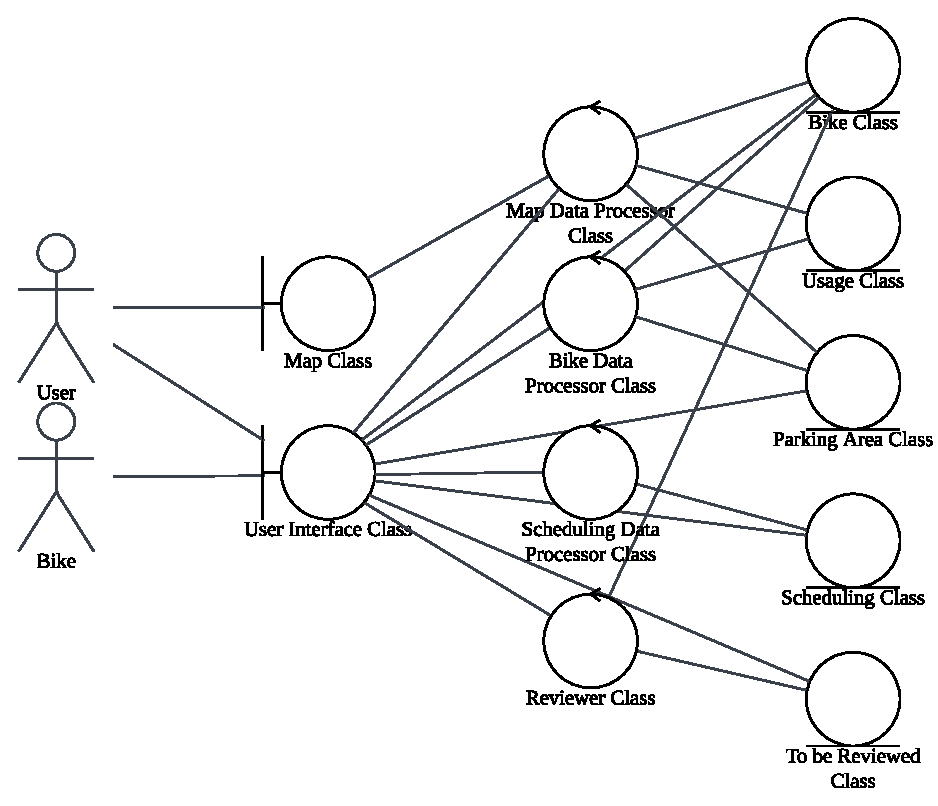
\includegraphics[width=\textwidth]{figures/class.pdf}
%     \caption{类图}\label{class}
% \end{figure}

\section{具体功能编写}
%简单介绍系统编写过程
在本项目的开发过程中,我们先使用Adobe XD来确定整个系统前端的设计和交互逻辑,然后使用Tailwind CSS和NextUI来
快速搭建出前端页面。

对于后端开发,由于本项目所采用的是Typescript语言,所以我首先根据数据字典来编写包含本项目所需类型定义的文件\verb|src\lib\definitions.ts|。
在此基础之上,再根据数据流图编写数据访问层对应文件\verb|src\lib\dal.ts|。最后,根据用例中描述的逻辑来实现业务逻辑,在此过程中完成Server Actions对应文件
\verb|src\lib\actions.ts|的编写。当然,在实际的开发过程中,上述三个部分相互之间是穿插着进行的,但是大体流程仍是分为上述三个阶段。

特别地,我在数据库中创建以下用户自定义函数:

\begin{enumerate}
    \item \texttt{create\_manager}:用户创建管理员账号;
    \item \texttt{create\_analyst}:用于创建分析团队账号;
    \item \texttt{check\_password}:用于检查账号和密码是否正确;
    \item \texttt{mark\_low\_battery}:用于全局更新“低电量”状态;
    \item \texttt{mark\_idle\_bikes}:用于全局更新“闲置”状态;
    \item \texttt{update\_luflt\_status}:用于全局更新“长期未关锁”状态;
    \item \texttt{update\_outdated\_status}:用于全局更新“型号老旧”状态;
    \item \texttt{update\_on\_parking\_area\_change}:给定停车区域数据,更新与该数据相关的\verb|contain|表中的数据,以及“违规停车”状态;
    \item \texttt{update\_on\_bike\_change}:给定单车数据,更新与该数据相关的\verb|contain|表中的数据,以及“违规停车”状态;
\end{enumerate}

同时,我在数据库中创建了以下触发器:

\begin{enumerate}
    \item \texttt{trigger\_parking\_area}:当管理创建、删除或更新停车区域数据时,自动对涉及数据调用 \texttt{update\_on\_parking\_area\_change}来维护一致性;
    \item \texttt{trigger\_bike}:当共享单车上传数据,或者管理员更新、创建或删除单车数据时,自动对涉及数据调用\texttt{update\_on\_bike\_change}来维护一致性;
\end{enumerate}

在项目开发末尾,我对本系统对于数据库的交互进行了统计分析。并对频繁用于连接和条件查询的域建立了索引。


\begin{table}
\centering
\caption{索引}
\label{index}
\begin{tabular}{ll}\toprule
  索引名&索引对象\\\midrule
  \texttt{idx\_scheduling}&\textit{\textbf{scheduling}(bike\_id)}\\
  \texttt{idx\_bike\_status}&\textit{\textbf{bike\_status}(bike\_id)}\\
  \texttt{idx\_parking\_area}&\textit{\textbf{parking\_area}(parking\_area\_id)}\\
  \texttt{idx\_bike}&\textit{\textbf{bike}(bike\_id)}\\
  \texttt{idx\_to\_be\_reviewed\_status}&\textit{\textbf{to\_be\_reviewed\_status}(bike\_id,time)}\\
  \texttt{idx\_to\_be\_reviewed\_proof\_material}&\textit{\textbf{to\_be\_reviewed\_proof\_material}(bike\_id,time)}\\
  \texttt{idx\_to\_be\_reviewed}&\textit{\textbf{to\_be\_reviewed}(bike\_id,time)}\\
  \texttt{idx\_usage}&\textit{\textbf{usage}(bike\_id)}\\
  \texttt{idx\_contain}&\textit{\textbf{contain}(bike\_id)}\\
  \texttt{idx\_contain\_}&\textit{\textbf{contain}(parking\_area\_id)}\\
 \bottomrule
\end{tabular}
\end{table}

\section{功能测试}
% %对编写系统进行实际测试
我对系统进行两方面的测试:

\begin{enumerate}
    \item 以摩拜共享单车2017年8月的数据集为基础,构造数据,并对数据库进行填充,主要用于测试用例\texttt{Generate Bike Distribution Map},\texttt{Generate Parking Area Distribution Map},\texttt{Produce Bike Status Statistics},\texttt{Update Bike Status Globally};
    \item 使用空数据库,主要用于测试涉及插入操作的用例,如\texttt{Upload Scheduling Log},\texttt{Update Single Bike Status},\texttt{Produce Bike Scheduling Log},\texttt{Update Bike Information},\texttt{Modify Bike List},\texttt{Modify Parking Area List}。
\end{enumerate}

上述两个测试覆盖了本项目的所有用例。

系统成功通过测试,并无功能性缺陷,但是在响应时间方面还有提升空间。测试时系统页面如图\ref{dashboard}-\ref{reviewPage}所示。

\begin{figure}[!htbp]
    \centering
    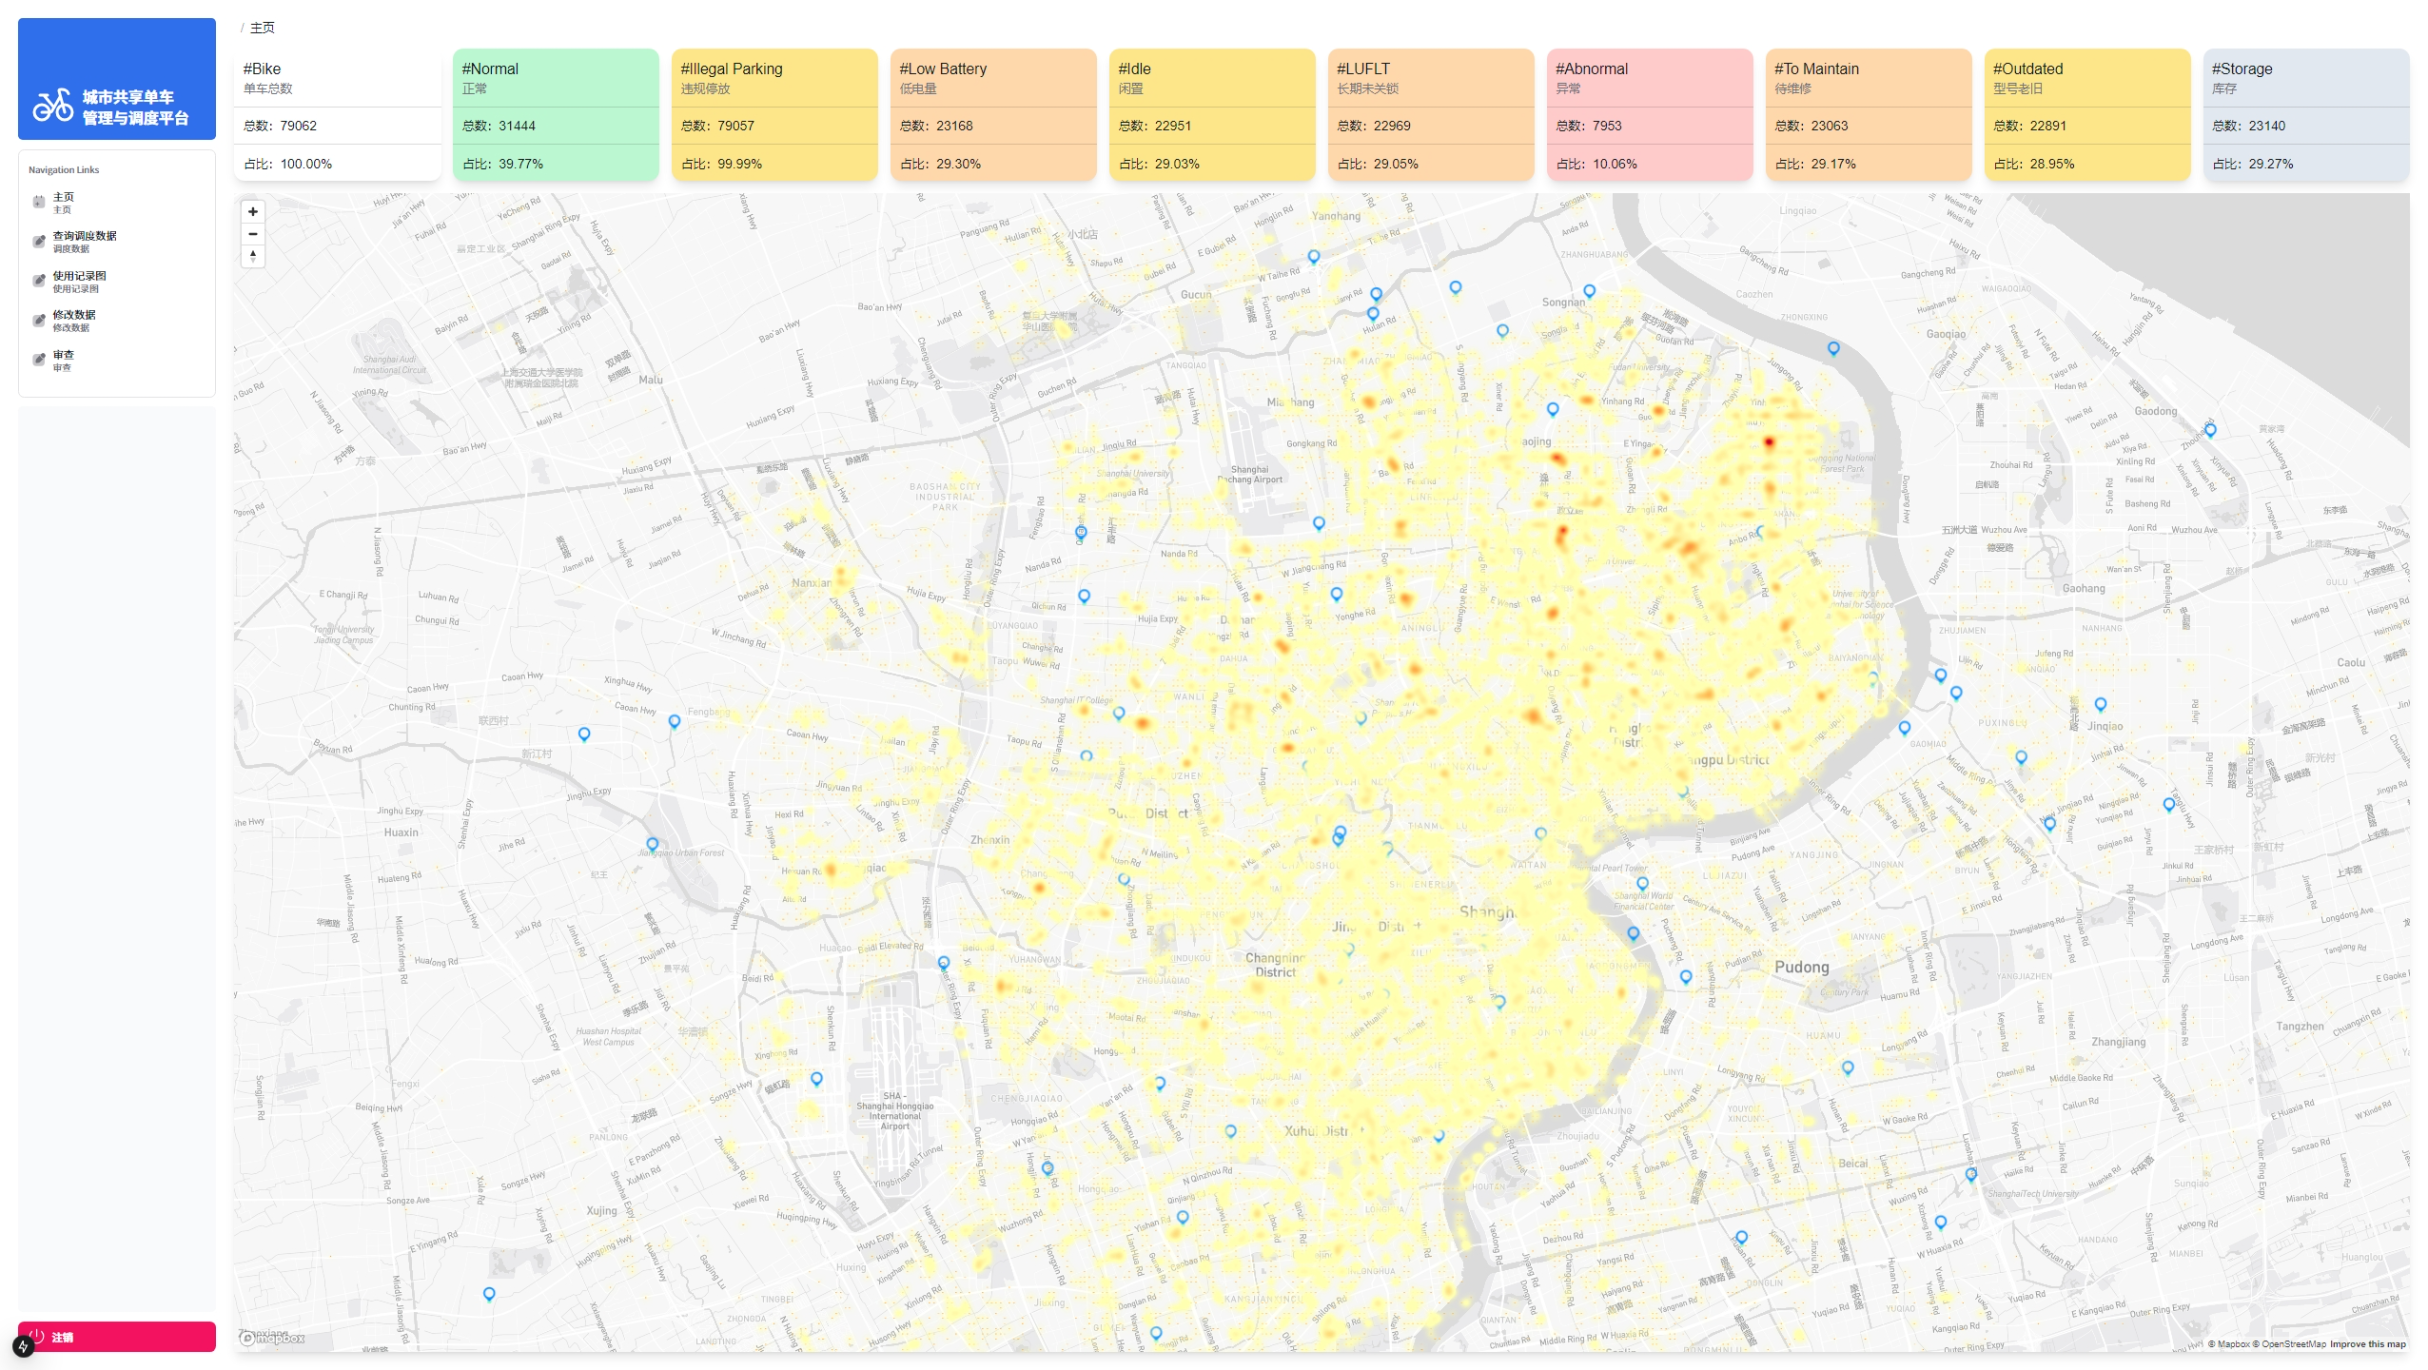
\includegraphics[width=\textwidth]{figures/dashboard.png}
    \caption{单车与停车区域分布图}\label{dashboard}
\end{figure}

\begin{figure}[!htbp]
    \centering
    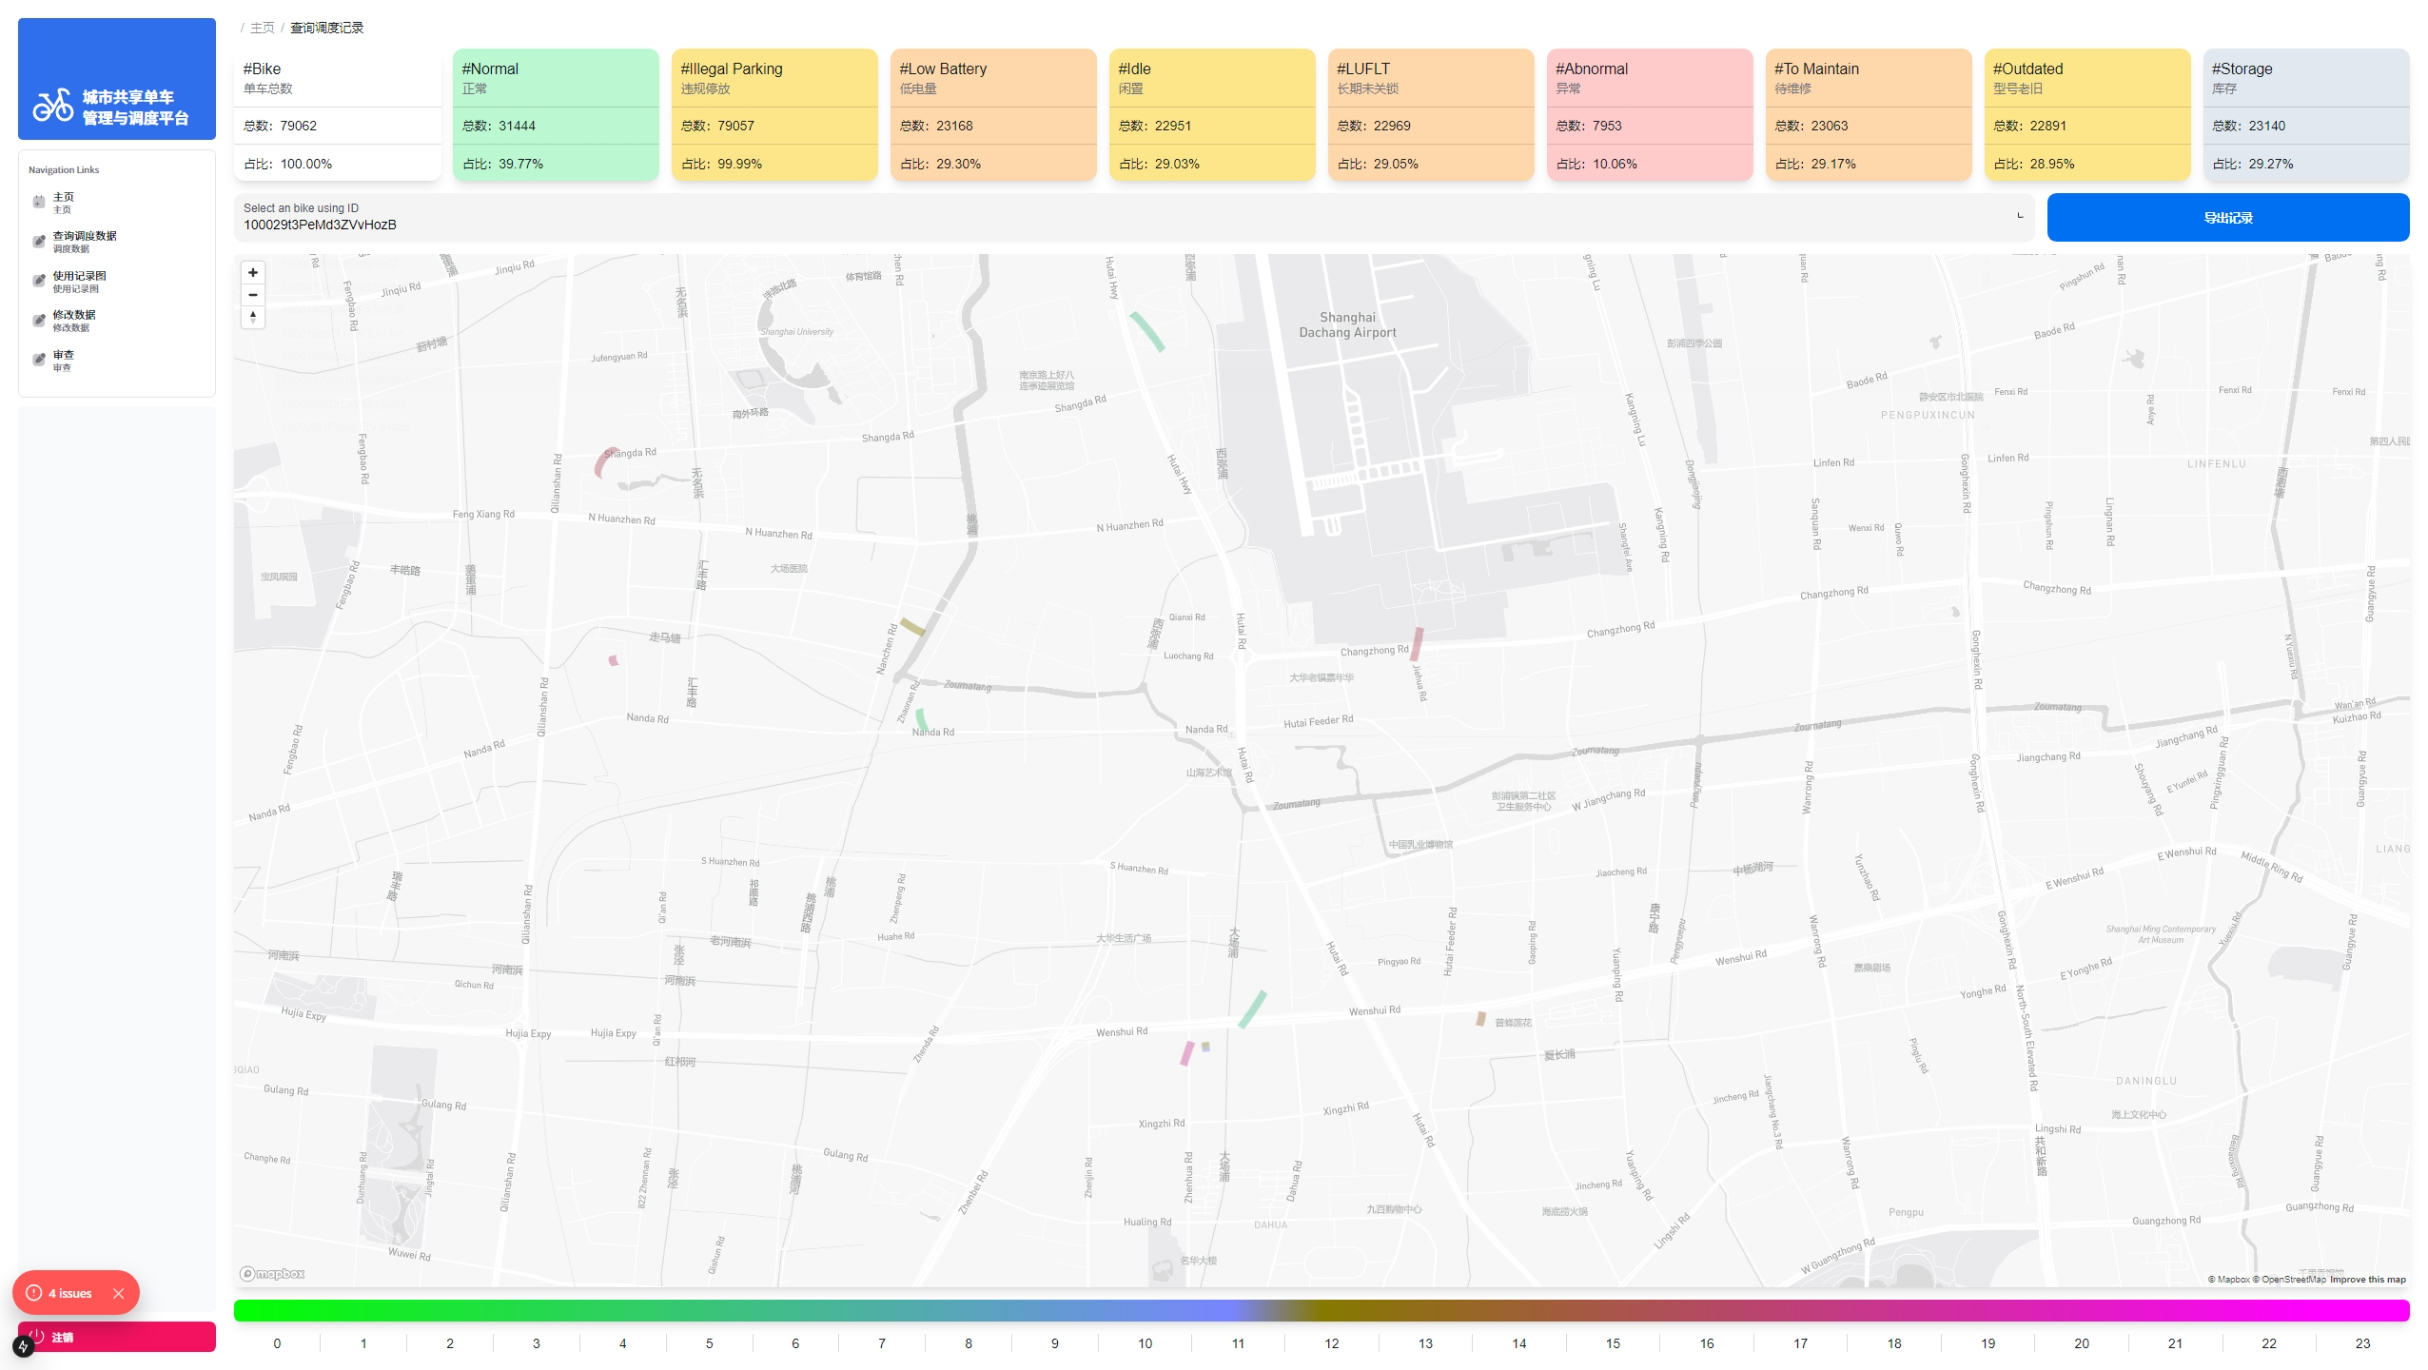
\includegraphics[width=\textwidth]{figures/schedule.png}
    \caption{单车调度记录图}\label{schedule}
\end{figure}

\begin{figure}[!htbp]
    \centering
    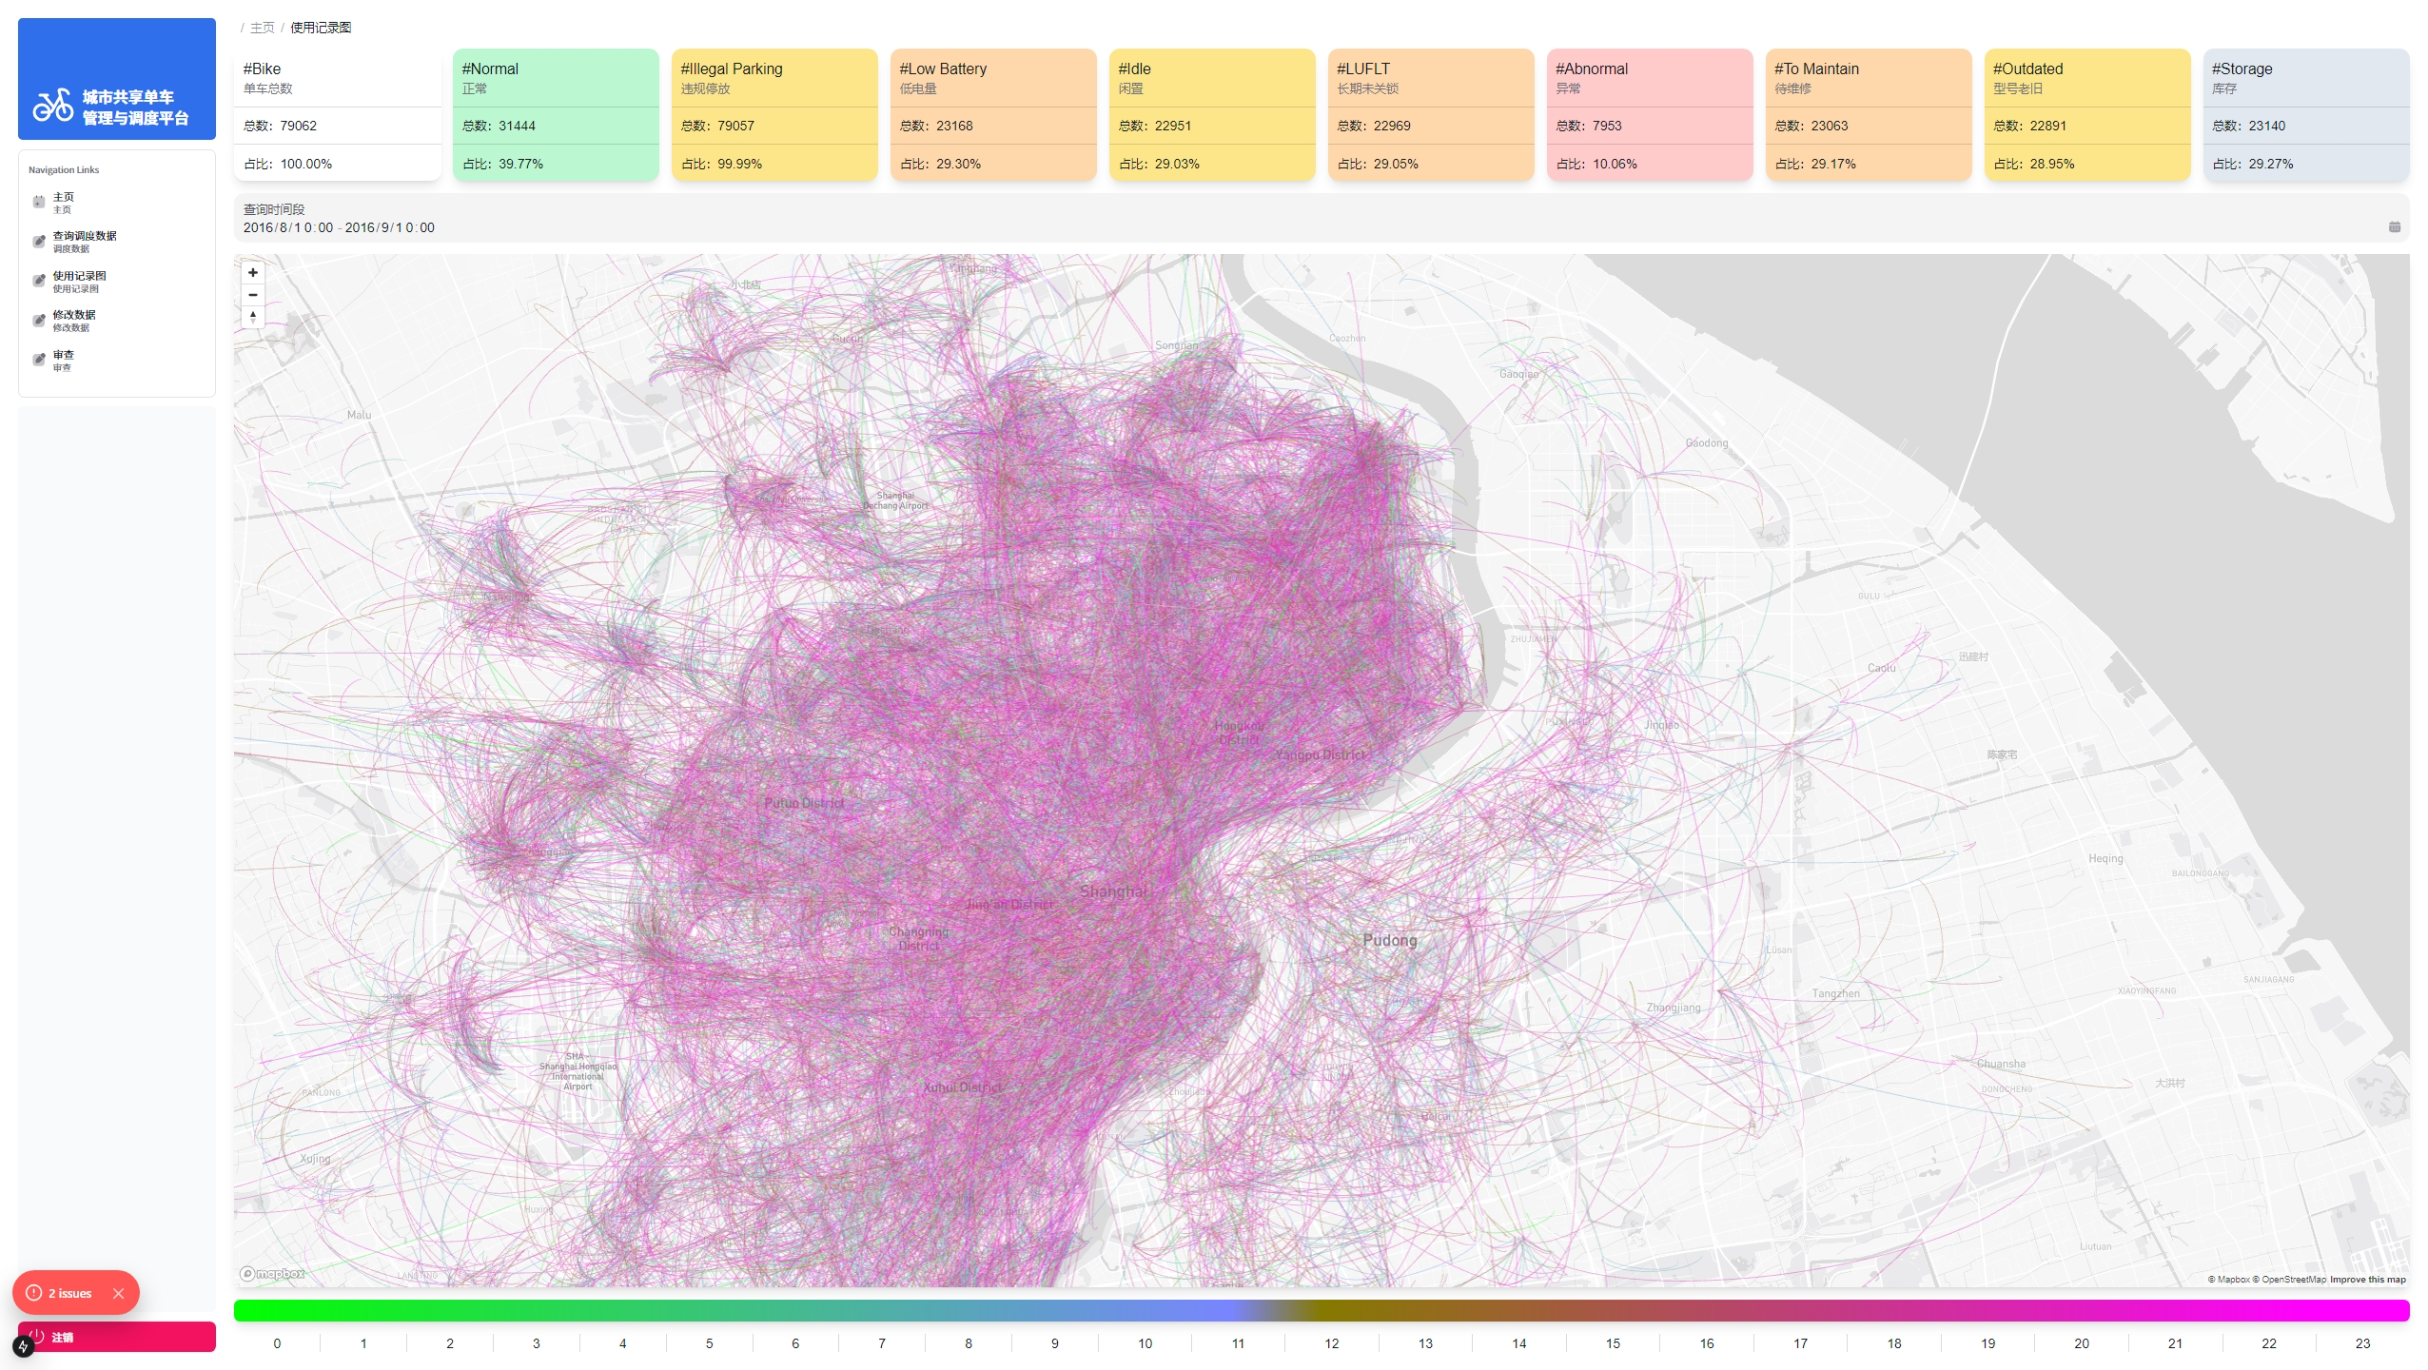
\includegraphics[width=\textwidth]{figures/usage.png}
    \caption{单车使用图}\label{usagePage}
\end{figure}

\begin{figure}[!htbp]
    \centering
    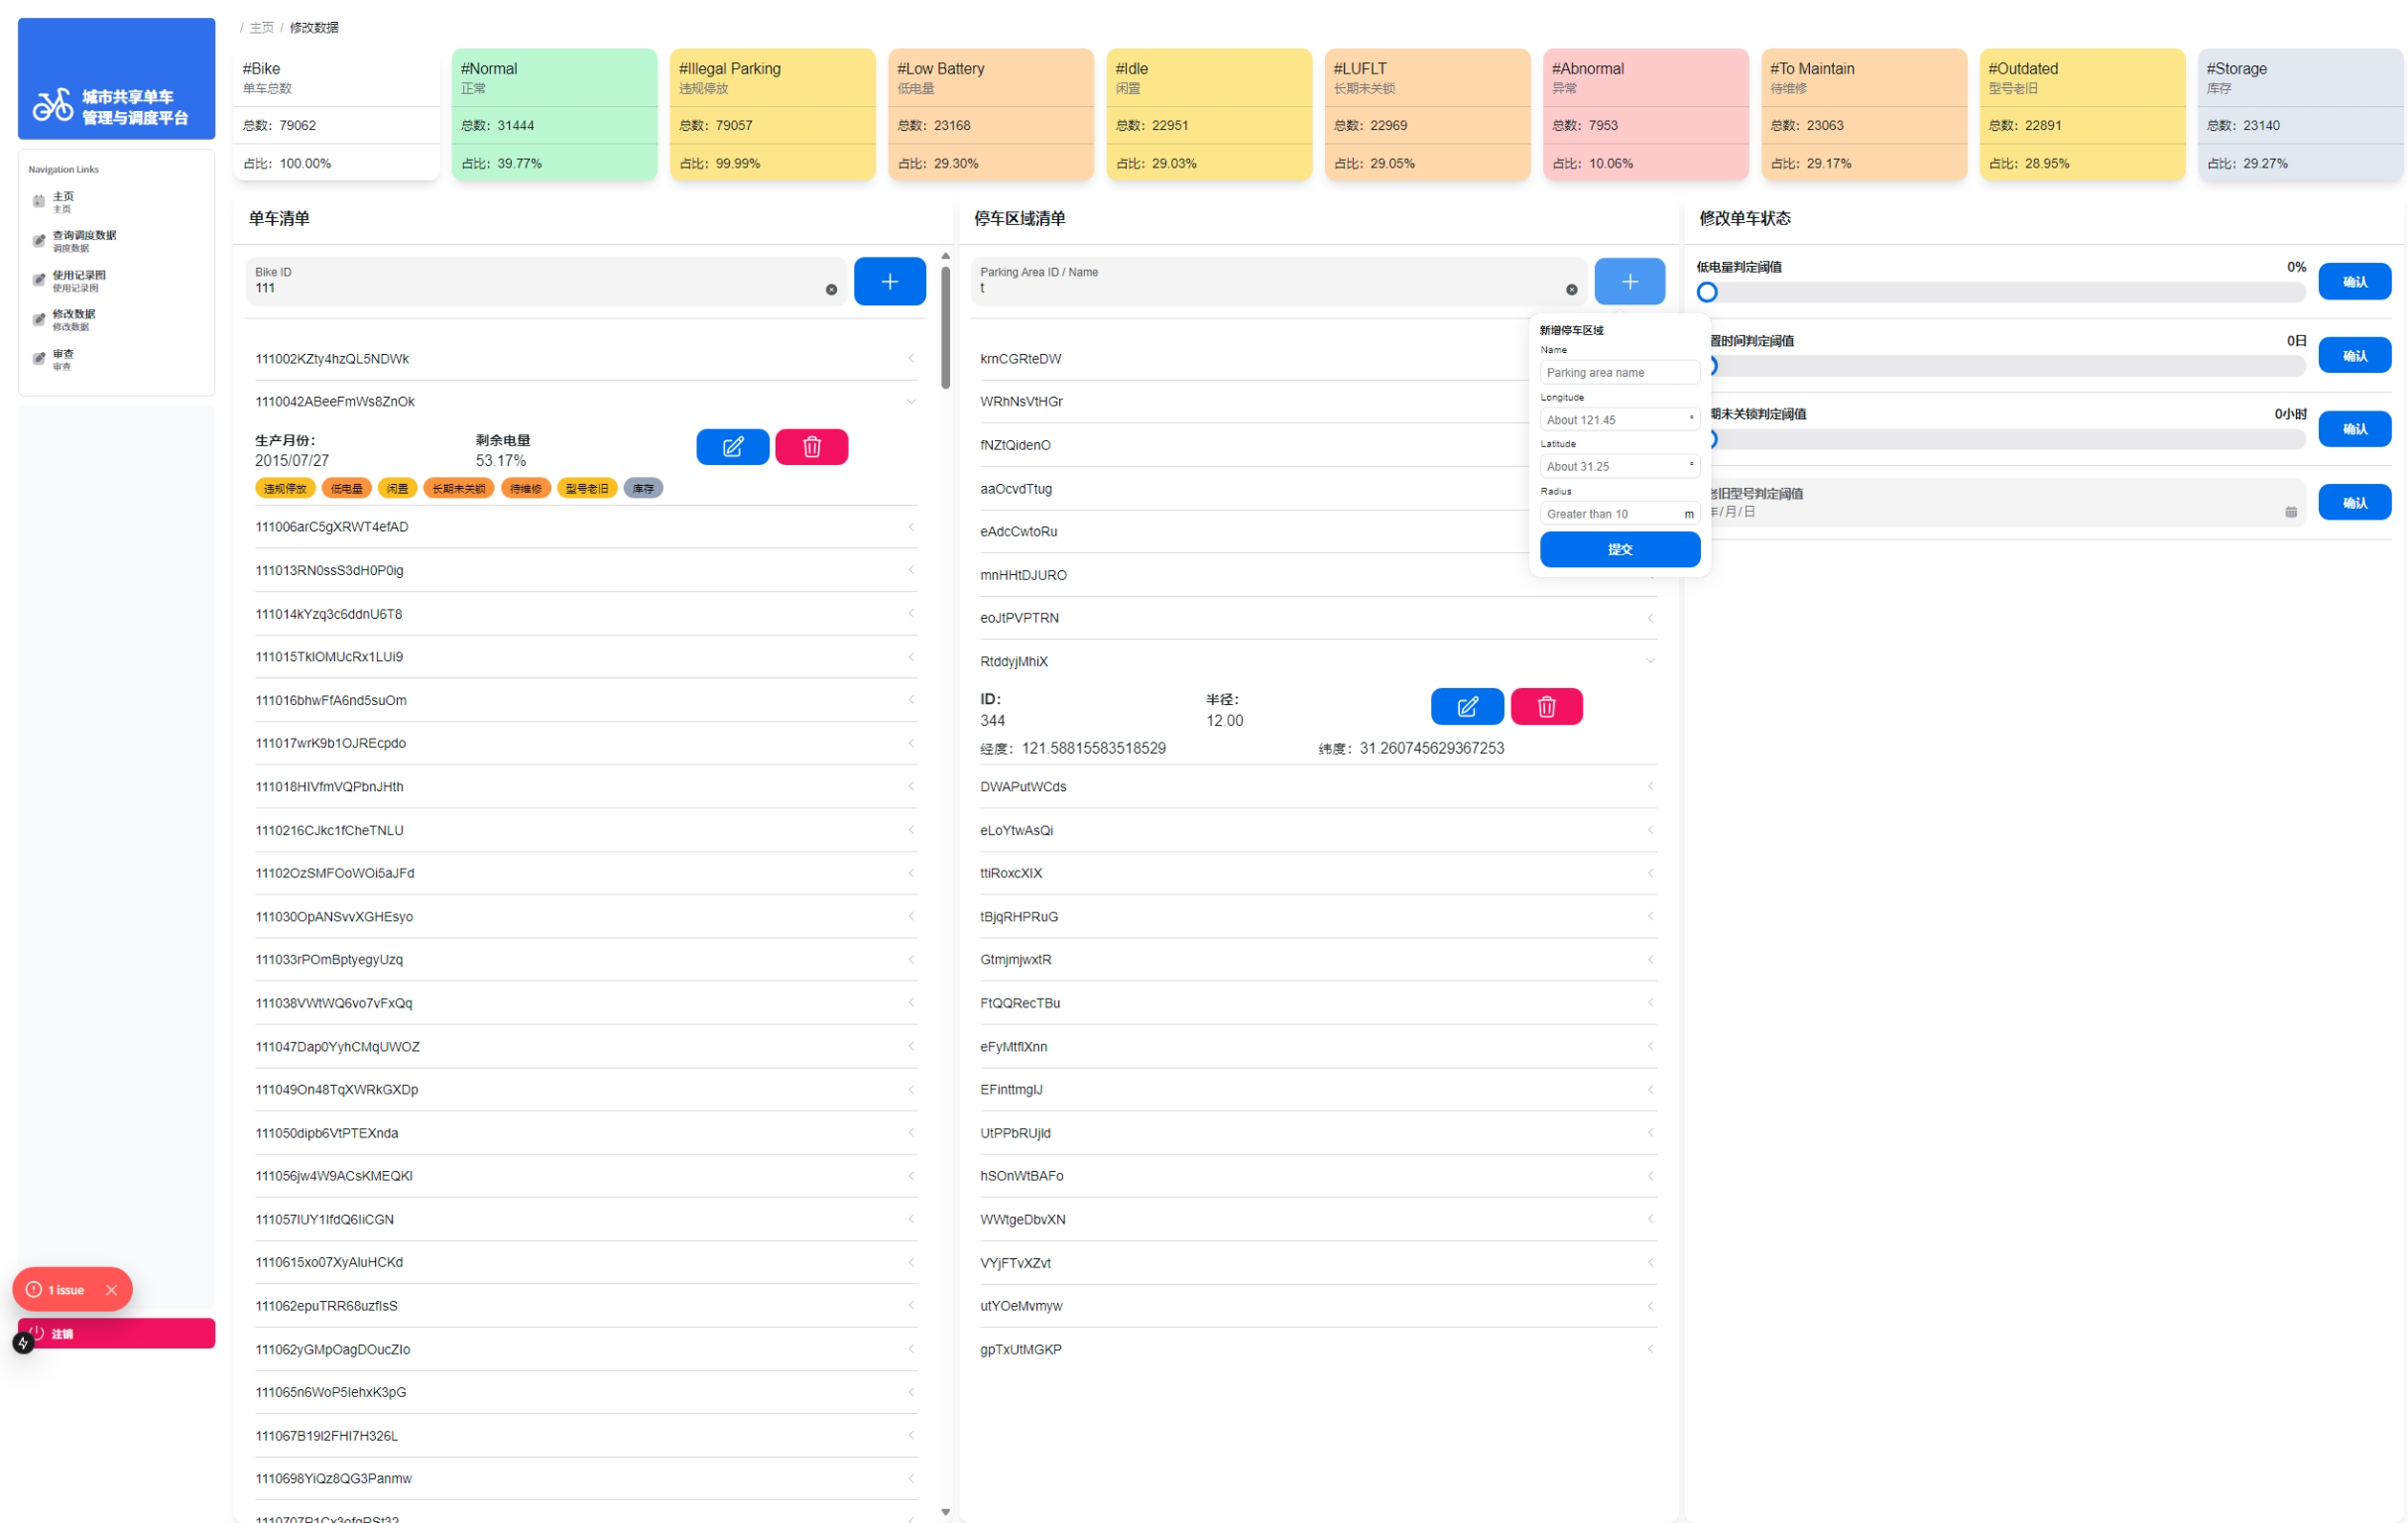
\includegraphics[width=\textwidth]{figures/modify.png}
    \caption{修改页面}\label{modify}
\end{figure}

\begin{figure}[!htbp]
    \centering
    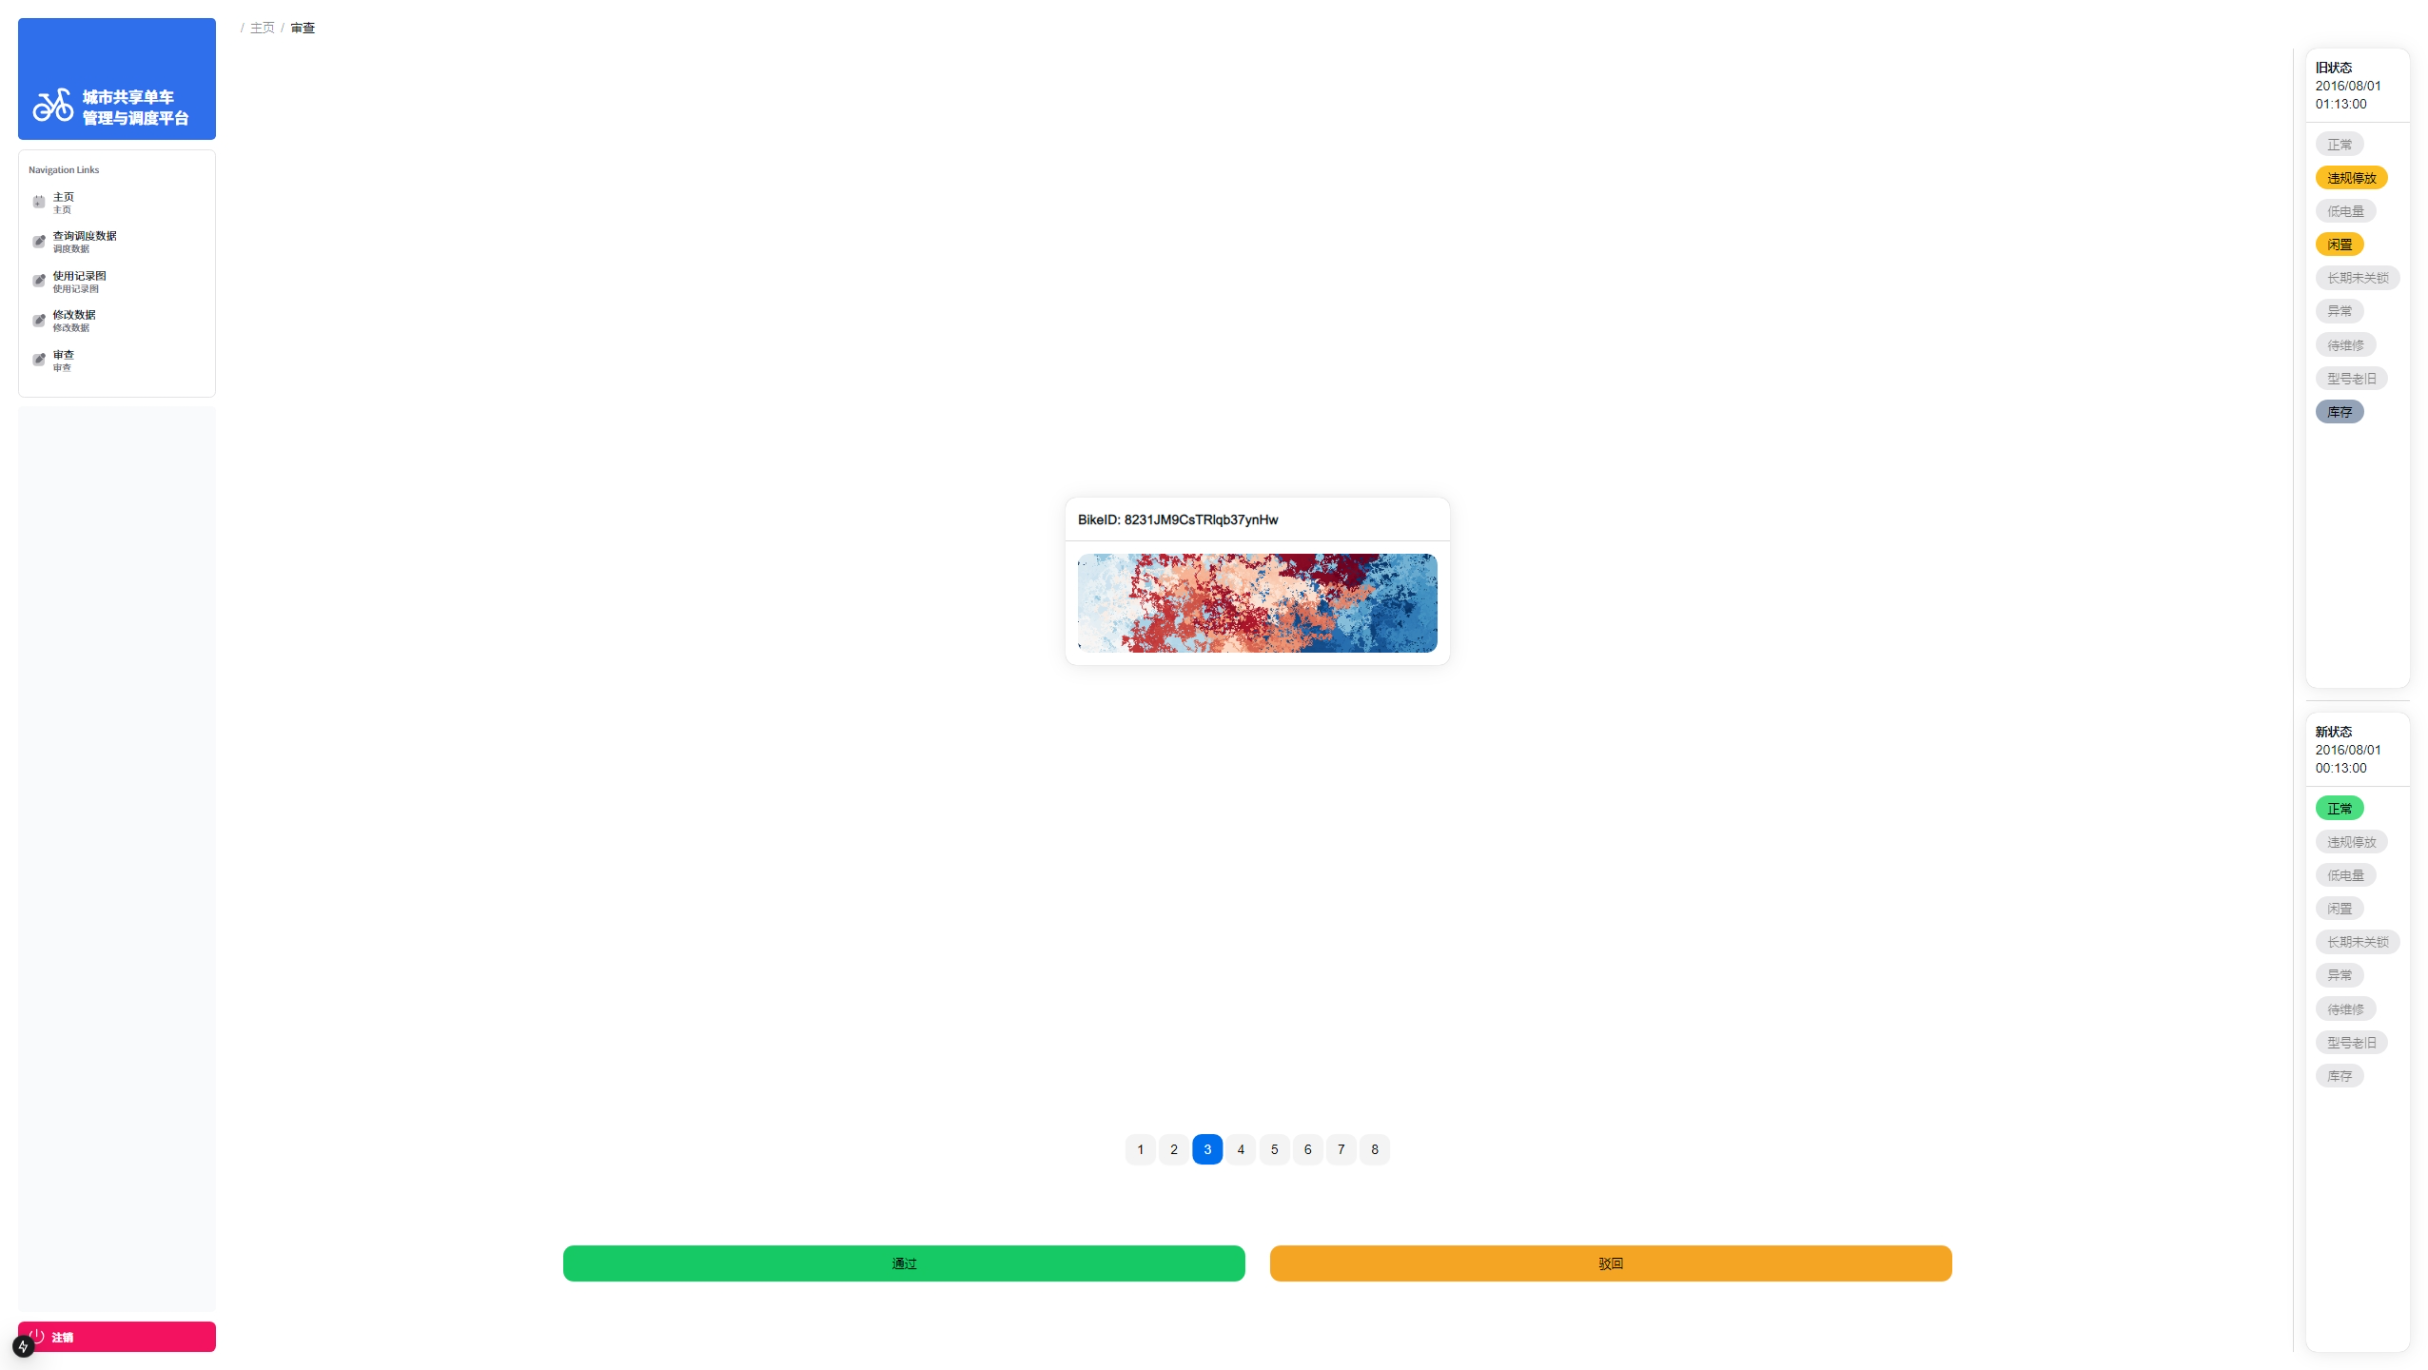
\includegraphics[width=\textwidth]{figures/review.png}
    \caption{审查页面}\label{reviewPage}
\end{figure}
